\begin{frame}[fragile]{Decision Problems}

\begin{center}

\begin{tikzpicture}
\matrix (m) [matrix of nodes,row sep=0.2em,column sep=0.2em,minimum width=2em]
  {
       \begin{minipage}[t]{.45\textwidth}
       \begin{center}
     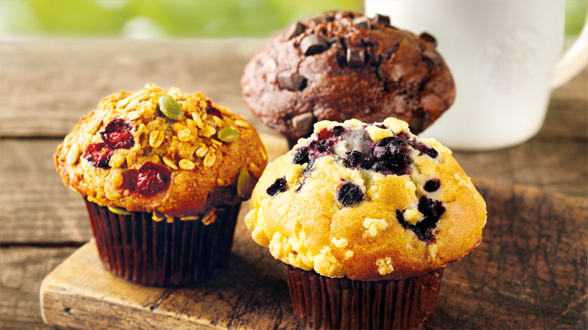
\includegraphics[width=.7\textwidth]{img/muffins.jpg} \\
     ``How many muffins of each kind?''
     \end{center}
     \end{minipage} 
       & 
     \begin{minipage}[t]{.5\textwidth}     
     \begin{center}
     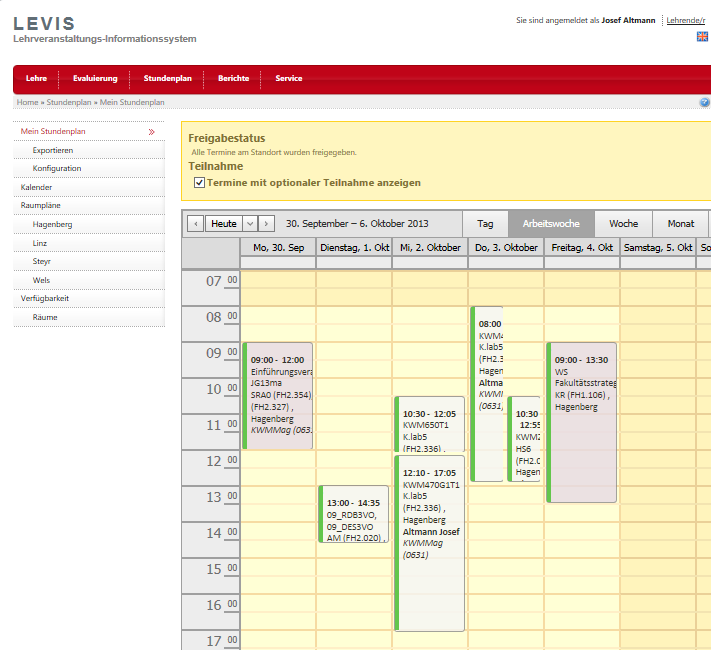
\includegraphics[width=.45\textwidth]{img/levis.png} \\
     ``When does which lecture take place?''     
       \end{center}
     \end{minipage}  \\
     \begin{minipage}[t]{.45\textwidth}     
     \begin{center}
     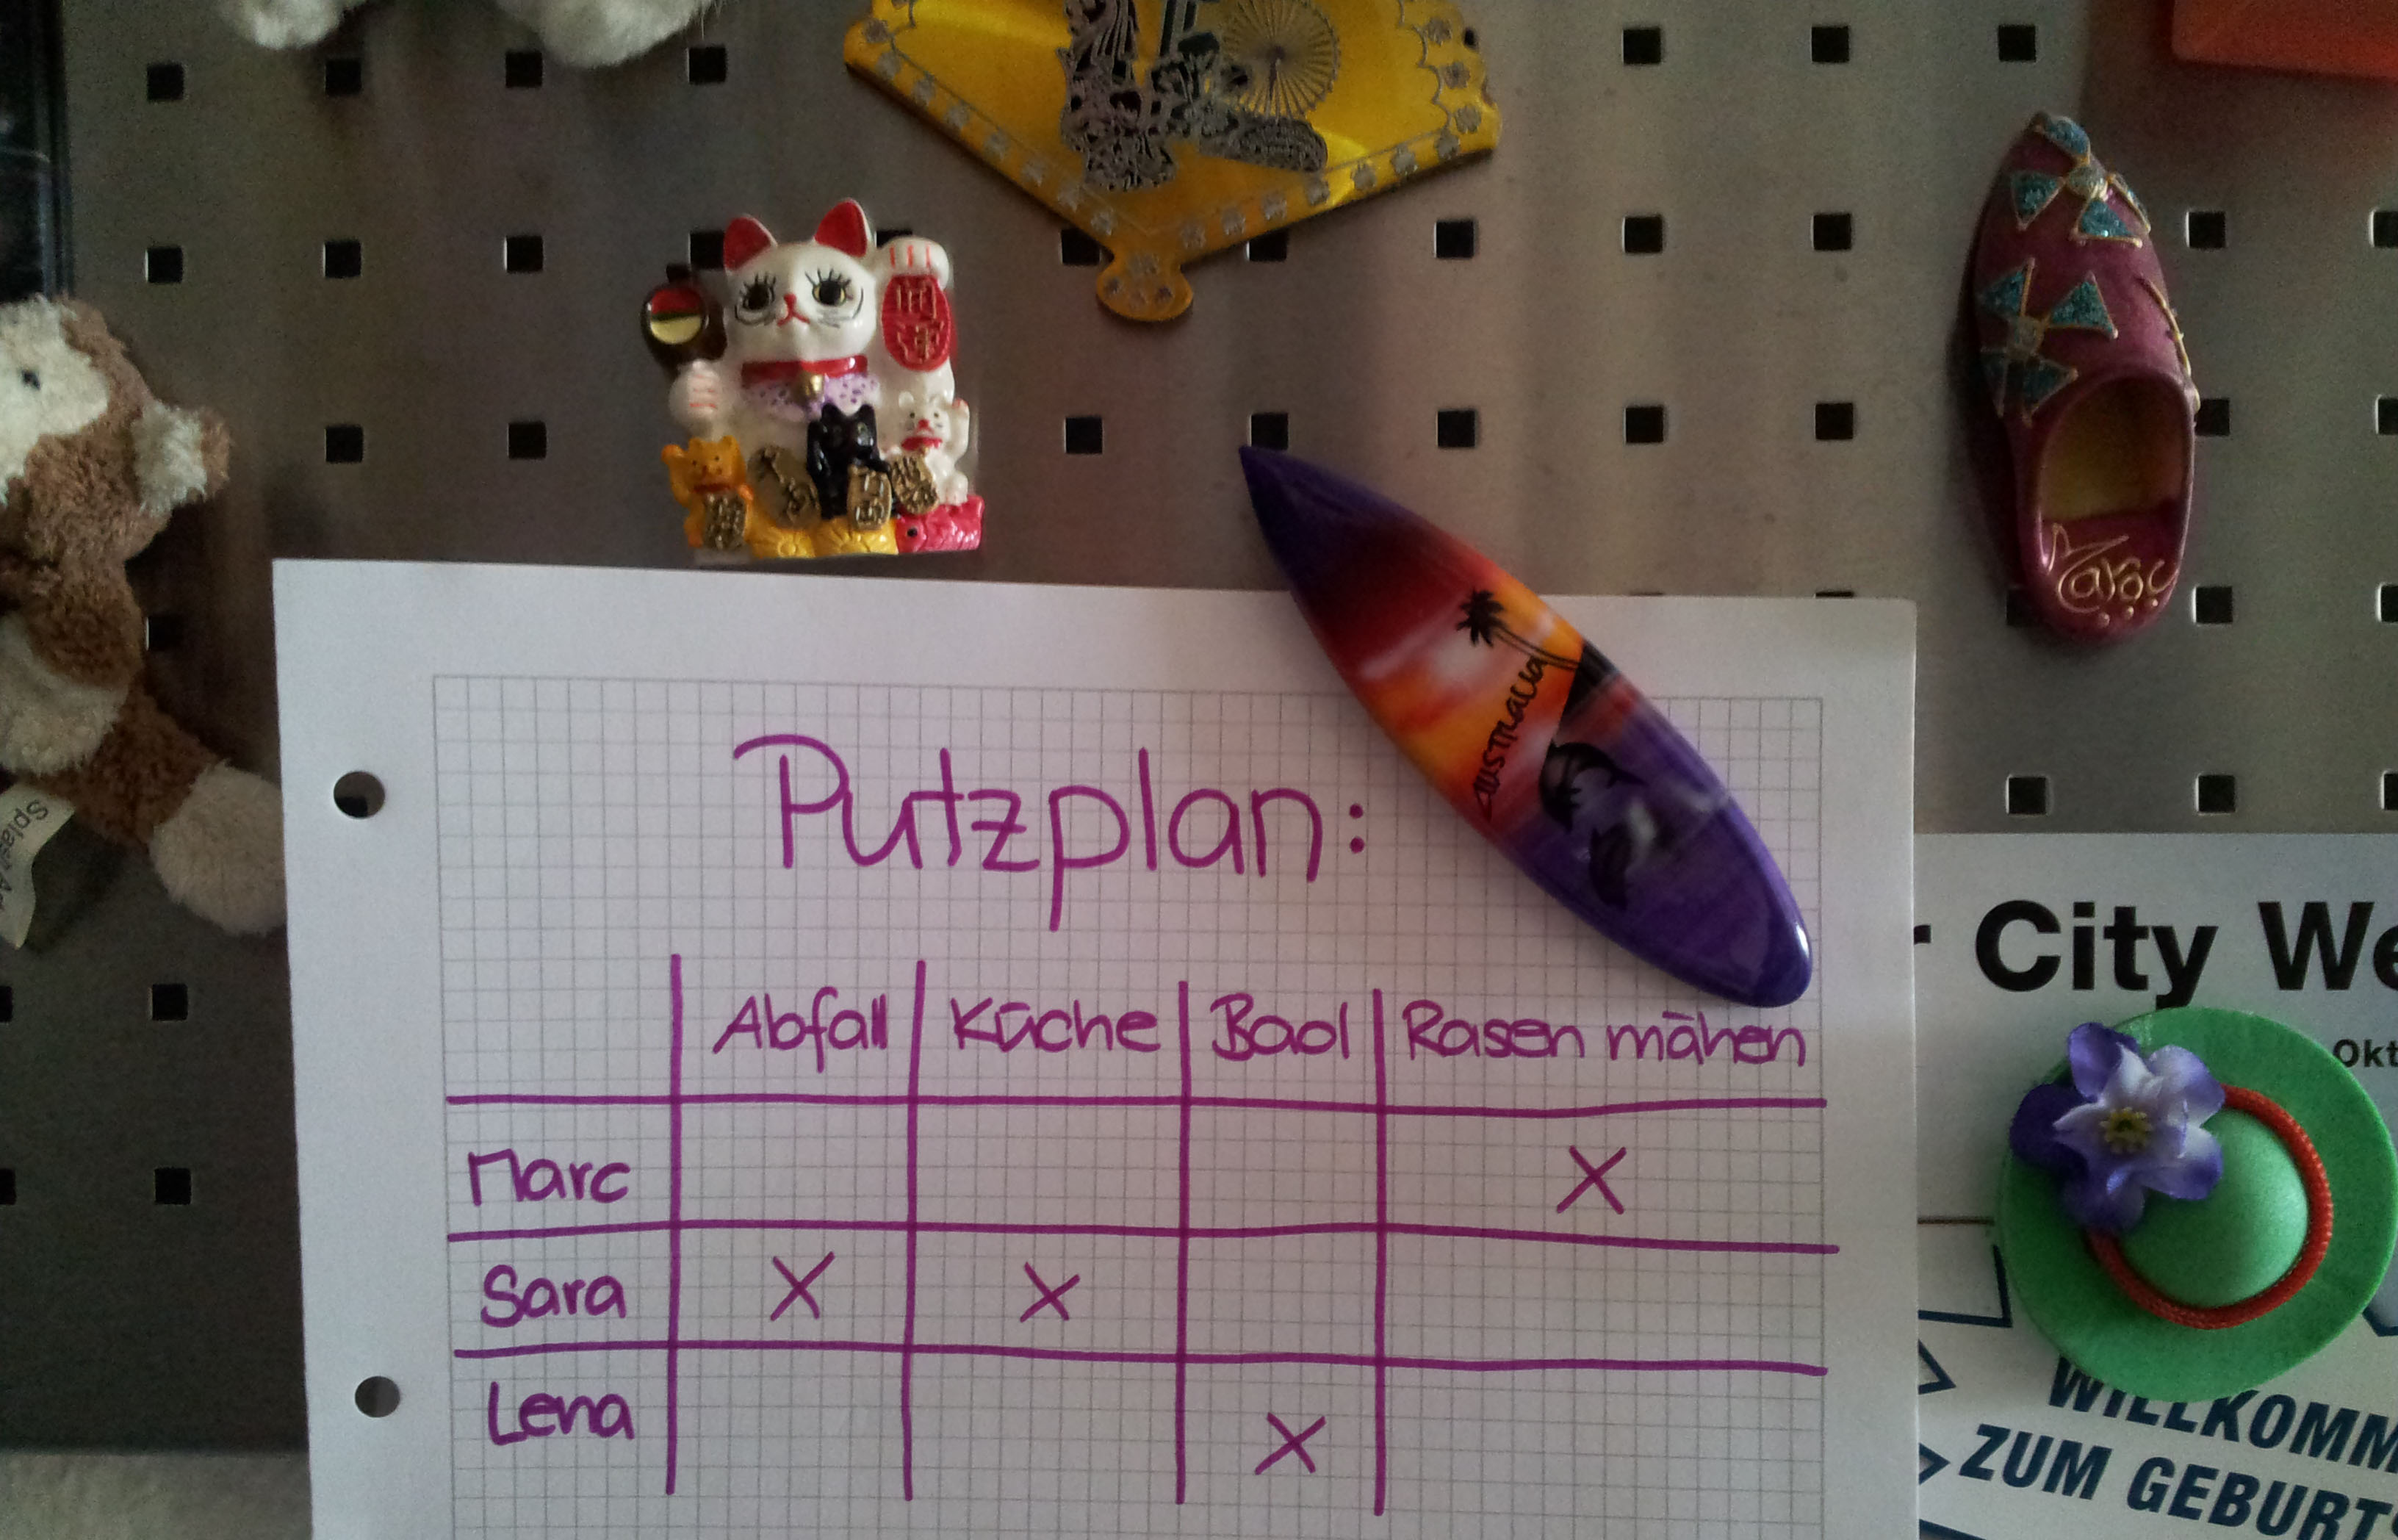
\includegraphics[width=.7\textwidth]{img/putzplan.jpg} \\
     ``Who performs which tasks?''
       \end{center}
     \end{minipage}  & 
     
     \begin{minipage}[t]{.45\textwidth}
     \begin{center}
           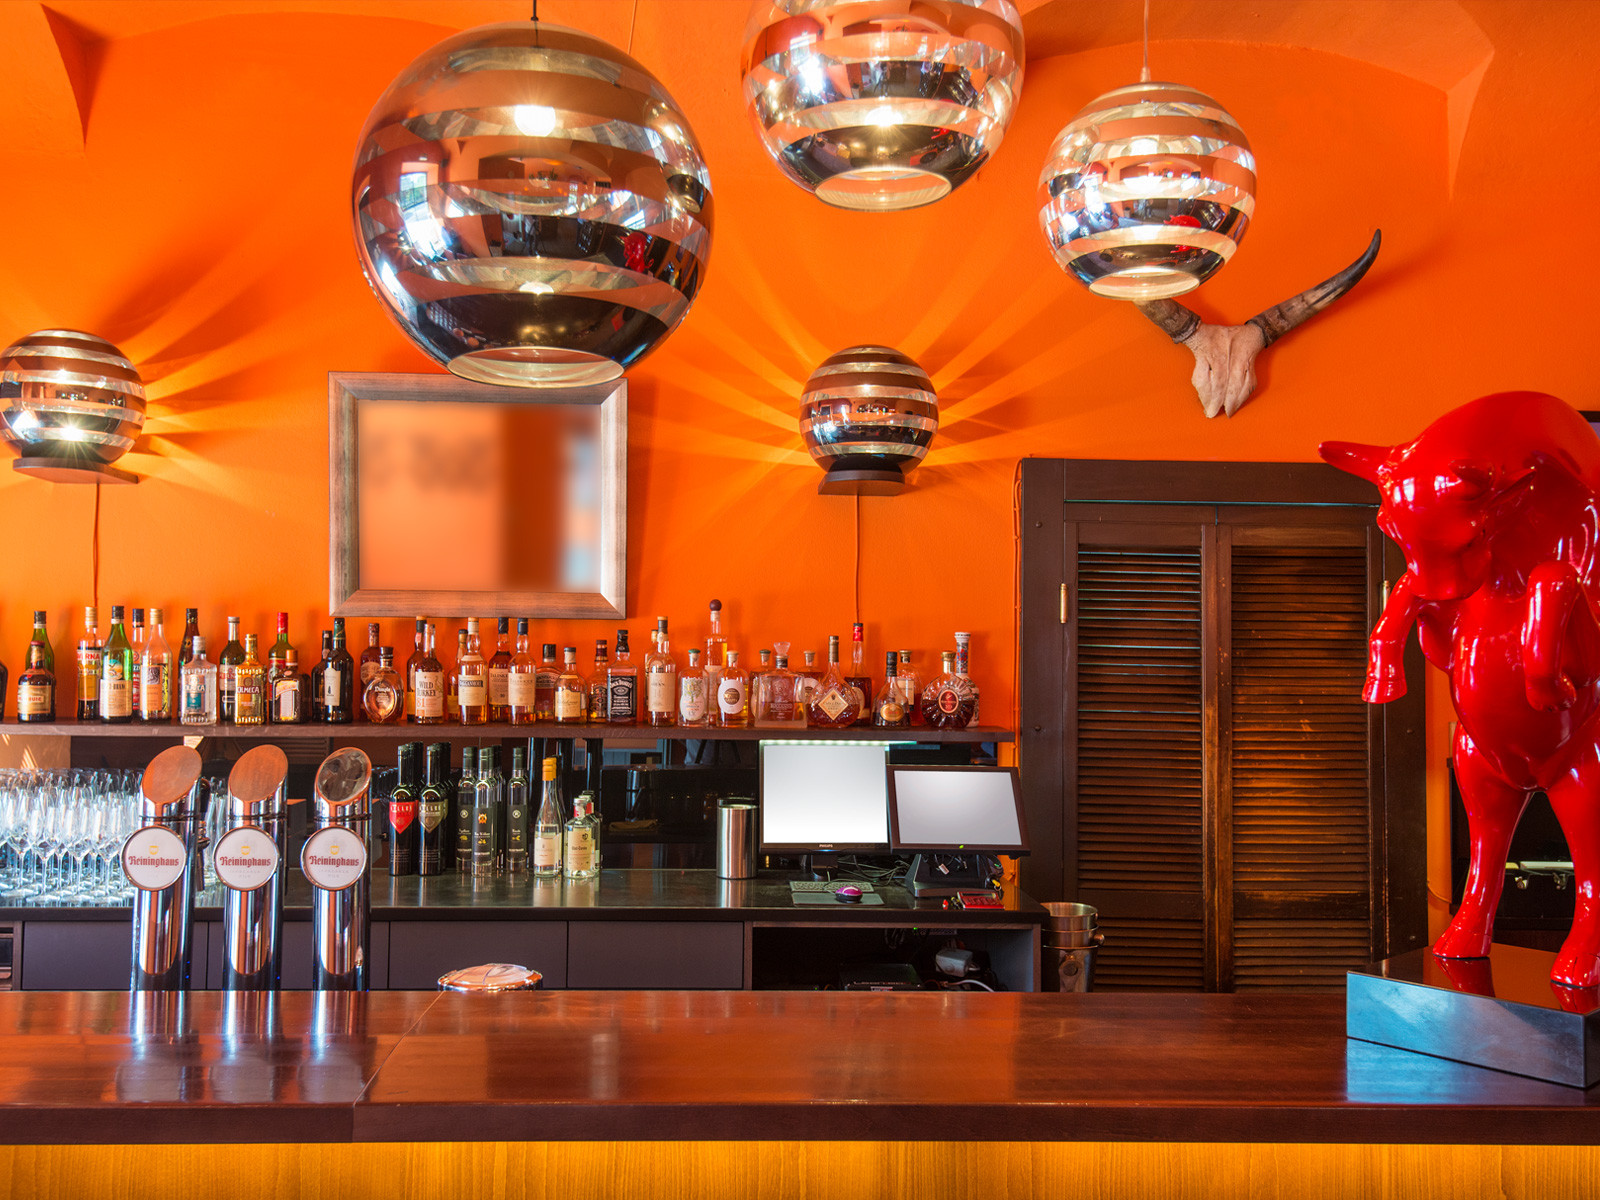
\includegraphics[width=.7\textwidth]{img/resti.jpg} \\
           ``What's up on the weekend?'' 
       \end{center}
     \end{minipage}
\\};
     
%  \path[-stealth]
%    (m-1-1) edge node [left] {$\mathcal{B}_X$} (m-2-1)
%            edge [double] node [below] {$\mathcal{B}_t$} (m-1-2)
%    (m-2-1.east|-m-2-2) edge node [below] {$\mathcal{B}_T$}
%            node [above] {$\exists$} (m-2-2)
%    (m-1-2) edge node [right] {$\mathcal{B}_T$} (m-2-2)
%            edge [dashed,-] (m-2-1);
\end{tikzpicture}

\end{center}
\end{frame}

\begin{frame}{What do these problems have in common?}
\hFirst{Decisions} \onslide<2->{\emph{(variables)}}
\begin{itemize}
\item The number of chocolate or banana muffins
\item The lectures in the curriculum
\item Friday and saturday activity
\end{itemize}
\pause

\vspace*{2ex}

\hFirst{Possibilities} \onslide<3->{\emph{(domains)}}
\begin{itemize}
\item Chocolate muffins: $\{0, \ldots, 20\}$
\item Lecture ``Algorithms 101'': $\{\mathrm{LH1}, \mathrm{LH2}, \mathrm{LH3}, \ldots \}$
\end{itemize}

\pause

\vspace*{2ex}

\hFirst{Dependencies} \onslide<4->{\emph{(constraints)}}
\begin{itemize}
\item The required flour for $x$ chocolate and $y$ banana muffins may not exceed 250g.
\item There can only be one class per room (at a time).
\item There can only be one all-you-can-eat buffet per weekend.
\end{itemize} \pause 
\end{frame}

\begin{frame}{What do these problems have in common?}
\hFirst{Preferences} \onslide<2->{\emph{(soft constraints)}}
\begin{itemize}
\item There \emph{should} be no algorithm lab on Friday, 8am
\item Bernd would like to have steaks, Ada prefers sushi $\rightarrow$ Ada's preference is \emph{more important}
\item I'd rather not clean nor vacuum. But if I have to do either, cleaning is \emph{worse}
\end{itemize}
\pause

\vspace*{2ex}
and/or
\vspace*{2ex}

\hFirst{Goals} \onslide<3->{\emph{(utility functions)}}
\begin{itemize}
\item Maximize the revenue of our chocolate/banana mix
\item Maximize the number of lecture-free days 
\end{itemize}

\vspace*{2ex}
\hfill a \alert{constraint satisfaction (optimization) problem} (CSP/COP), 

\hfill discrete if some decisions are over integers 
\end{frame}


\begin{frame}{Discrete Optimization Problems in FAS* (1)}

\begin{center}
Adaptive production cells

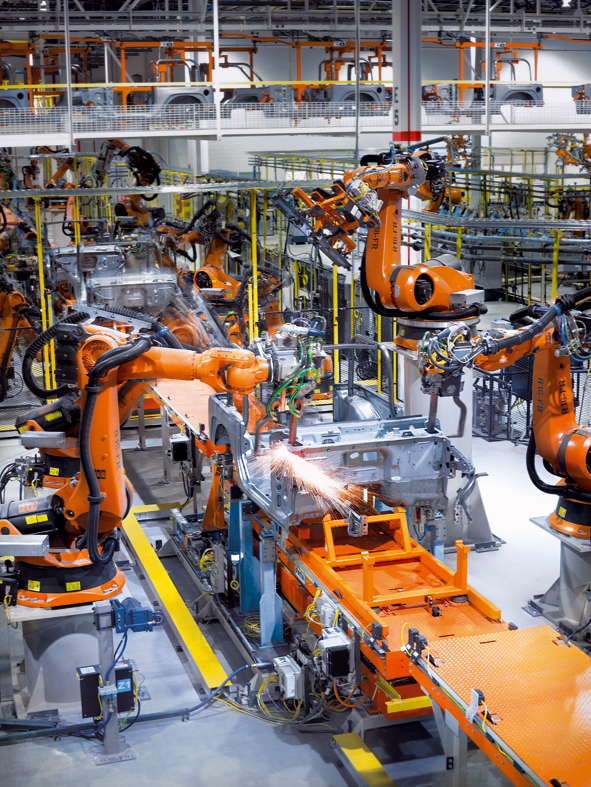
\includegraphics[width=.42\textwidth]{img/automobilindustrie.jpg}
\end{center}
\end{frame}

\begin{frame}{Discrete Optimization Problems in FAS* (1)}
\textbf{Goal}: Assign tasks to robots such that a correct \alert{resource flow} emerges
\begin{center}
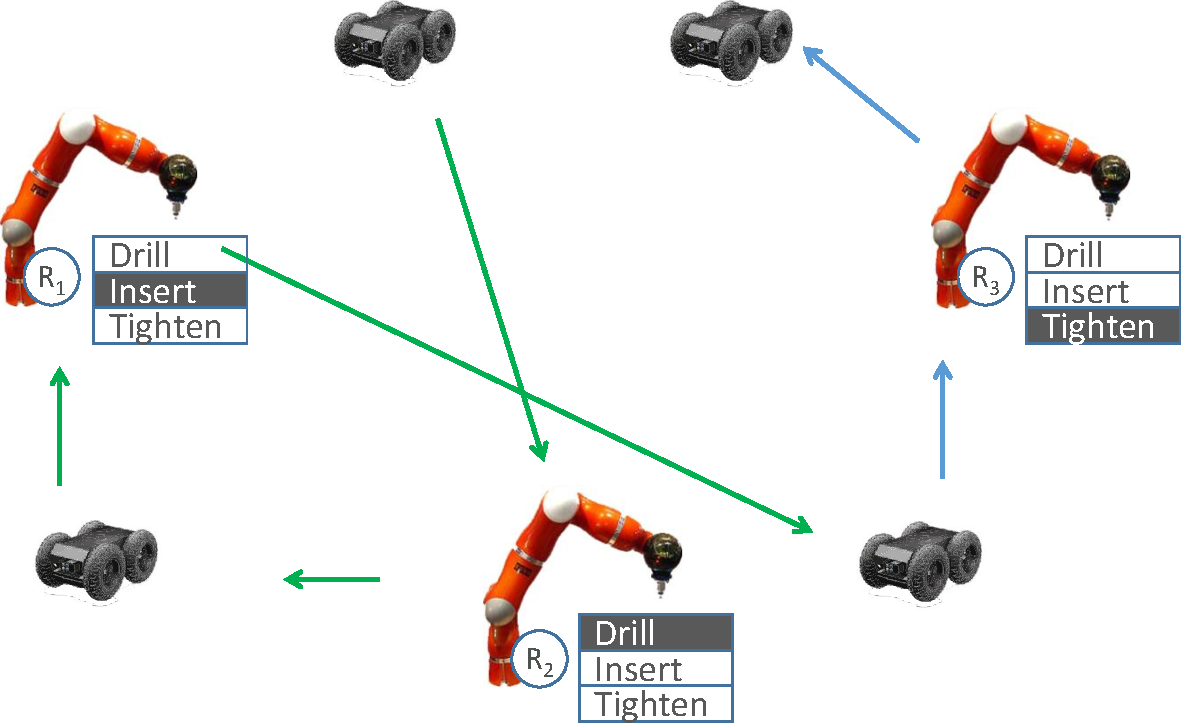
\includegraphics[width=.7\textwidth]{img/produktionszelle.pdf}
\end{center}

\hfill \cite{seebach2010software}, SASO

\end{frame}


\begin{frame}{Discrete Optimization Problems in FAS* (2)}
\begin{center}
Decentralized energy management
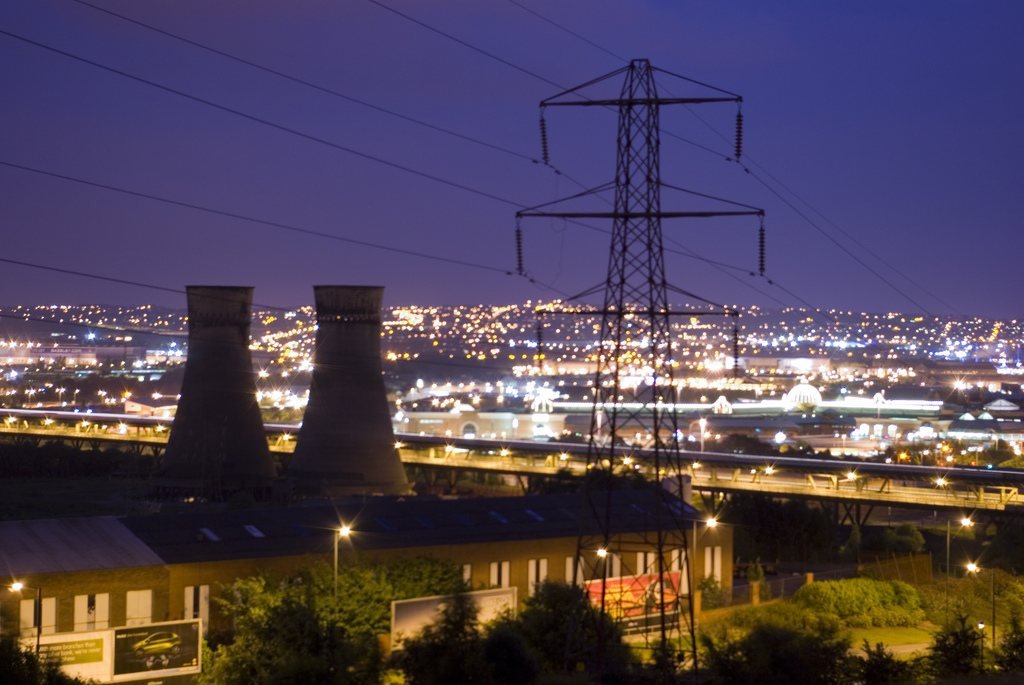
\includegraphics[width=.7\textwidth]{img/power_plants.jpg}
\end{center}
\end{frame}

\begin{frame}[fragile]{Discrete Optimization Problems in FAS* (2)}
\textbf{Goal}: Schedule power plants such that they meet the demand 
\tikzset{
    trajectory/.style={issegrey},
    emph/.style={isseorange},
    trajectorynode/.style={issegrey},
    demand/.style={MidnightBlue, thick},
    firstTraj/.style={ForestGreen},
    secTraj/.style={BrickRed}
} 
\begin{figure}
\begin{tikzpicture}[scale=1.0]
    % Draw axes
    \draw [<->,thick] (0,5) node (yaxis) [above] {$P(t)$}
        |- (8.5,0) node (xaxis) [right] {$t$};
        
    \node[overlay,text width=1.9cm, text centered, anchor=south, right] at (7.7,4.5)
    { \small 
    \begin{itemize} 
    \item[] { \color{MidnightBlue} \onslide<2->{\textbf{Demand}} } 
    \item[] { \color{ForestGreen} \onslide<3->{Plant $a$} } 
    \item[] { \color{BrickRed} \onslide<4->{Plant $b$} }  
    \item[] { \color{isseorange} \onslide<5->{\textbf{Supply}} }    
    \end{itemize}
    };        
       
	
%	\node[text width = 1.5cm ,text centered, anchor=west, right] at (2.5, 1)
%	{
%		$\mathbf{+}$
%	};
	
    %\node[text width=2.5cm, text centered, anchor=west, right] at (4,-.5)
    %{
    %		Kraftwerk $\mathsf{b}$
	%}; 
	
	%\node[text width = 1.5cm ,text centered, anchor=west, right] at (6.5, 1)
	%{
	%	$\mathbf{=}$
%	};
	%\node[text width=2.5cm, text centered, anchor=west, right] at (8,-.5)
    %{
    %		Demand
	%};      
    
     % draw second trajectory first graph 
     \onslide<2->{
    \draw[trajectory,demand] (0,3.9) coordinate (d20) -- (1,4.6) coordinate (d21);
    \draw[trajectory,demand] (d21) -- (2,4.4) coordinate (d22);
    \draw[trajectory,demand] (d22) -- (3,4.7) coordinate (d23);
    \draw[trajectory,demand] (d23) -- (4,3.5) coordinate (d24);
    \draw[trajectory,demand] (d24) -- (5,3.5) coordinate (d25);
    \draw[trajectory,demand] (d25) -- (6,3.5) coordinate (d26);
    \draw[trajectory,demand] (d26) -- (7,4.0) coordinate (d27);
    \draw[trajectory,demand] (d27) -- (8,4.5) coordinate (d28);
    
    % now for the circles
    \fill[trajectorynode,demand] (d21) circle (1pt);
    \fill[trajectorynode,demand] (d22) circle (1pt);
    \fill[trajectorynode,demand] (d23) circle (1pt);
    \fill[trajectorynode,demand] (d24) circle (1pt);    
    \fill[trajectorynode,demand] (d25) circle (1pt);
    \fill[trajectorynode,demand] (d26) circle (1pt);
    \fill[trajectorynode,demand] (d27) circle (1pt);
    \fill[trajectorynode,demand] (d28) circle (1pt);
    }
        
    \onslide<3->{
    % now for the first plant   
    \draw[trajectory,firstTraj] (0,1.9) coordinate (p10) -- (1,2.0) coordinate (p11);
    \draw[trajectory,firstTraj] (p11) -- (2,2.4) coordinate (p12);
    \draw[trajectory,firstTraj] (p12) -- (3,2.4) coordinate (p13);
    \draw[trajectory,firstTraj] (p13) -- (4,2.2) coordinate (p14);
    \draw[trajectory,firstTraj] (p14) -- (5,2.4) coordinate (p15);
    \draw[trajectory,firstTraj] (p15) -- (6,2.4) coordinate (p16);
    \draw[trajectory,firstTraj] (p16) -- (7,2.4) coordinate (p17);                   
    \draw[trajectory,firstTraj] (p17) -- (8,2.6) coordinate (p18);
    
    	\onslide<6>{
       \draw[trajectory,firstTraj,very thick] (p11) -- (p12);	
       \node[overlay,align=left,rectangle callout,%
             callout absolute pointer=(p11.west),xshift=-.5cm,yshift=-1.5cm,fill=isseorange!50] at (p12) {
            \scriptsize \textbf{Must} ramp up \\ \scriptsize due to inertia};
       
	}    
    
 	\onslide<8>{
       \draw[trajectory,firstTraj,very thick] (p15) -- (p16);	
       \draw[trajectory,firstTraj,very thick] (p16) -- (p17);
       
          \node[overlay,align=left,rectangle callout,%
             callout absolute pointer=(p16.north),xshift=-.5cm,yshift=0.55cm,fill=isseorange!50] at (p15) {
           \scriptsize  Wait 2 steps for \\ \scriptsize further ramp-up};
	} 
	
    % now for the circles of the first graph
    \fill[trajectorynode,firstTraj] (p11) circle (1pt);
    \fill[trajectorynode,firstTraj] (p12) circle (1pt);
    \fill[trajectorynode,firstTraj] (p13) circle (1pt);
    \fill[trajectorynode,firstTraj] (p14) circle (1pt);    
    \fill[trajectorynode,firstTraj] (p15) circle (1pt);
    \fill[trajectorynode,firstTraj] (p16) circle (1pt);
    \fill[trajectorynode,firstTraj] (p17) circle (1pt);
    \fill[trajectorynode,firstTraj] (p18) circle (1pt);        
    }
    
    \onslide<4->{
    % now for the second plant   
    \draw[trajectory,secTraj] (0,2.0) coordinate (p20) -- (1,2.6) coordinate (p21);
    \draw[trajectory,secTraj] (p21) -- (2,2.0) coordinate (p22);
    \draw[trajectory,secTraj] (p22) -- (3,2.2) coordinate (p23);
    \draw[trajectory,secTraj] (p23) -- (4,1.5) coordinate (p24);
    \draw[trajectory,secTraj] (p24) -- (5,1.4) coordinate (p25);
    \draw[trajectory,secTraj] (p25) -- (6,1.2) coordinate (p26);
    \draw[trajectory,secTraj] (p26) -- (7,1.6) coordinate (p27);                   
    \draw[trajectory,secTraj] (p27) -- (8,1.9) coordinate (p28);
	\onslide<6>{
       \draw[trajectory,secTraj,very thick] (p21) -- (p22);	
       \node[overlay,align=left,rectangle callout,%
             callout absolute pointer=(p21.north),xshift=+1cm,yshift=.5cm,fill=isseorange!50] at (p21) {
            \scriptsize Has to compensate};
	}    
	
	\onslide<7>{
       \draw[trajectory,secTraj,very thick] (p23) -- (p24);	
       \node[overlay,align=left,rectangle callout,%
             callout absolute pointer=(p24.south),xshift=+1cm,yshift=-.8cm,fill=isseorange!50] at (p24) {
             \scriptsize Cannot ramp down further};
	}    
    
     % now for the circles of the second graph
    \fill[trajectorynode,secTraj] (p21) circle (1pt);
    \fill[trajectorynode,secTraj] (p22) circle (1pt);
    \fill[trajectorynode,secTraj] (p23) circle (1pt);
    \fill[trajectorynode,secTraj] (p24) circle (1pt);    
    \fill[trajectorynode,secTraj] (p25) circle (1pt);
    \fill[trajectorynode,secTraj] (p26) circle (1pt);
    \fill[trajectorynode,secTraj] (p27) circle (1pt);
    \fill[trajectorynode,secTraj] (p28) circle (1pt);
    }
    
    \onslide<5->{
    % draw joint production first graph 
    \draw[trajectory,emph] (0,3.9) coordinate (s20) -- (1,4.6) coordinate (s21);
    \draw[trajectory,emph] (s21) -- (2,4.4) coordinate (s22);
    \draw[trajectory,emph] (s22) -- (3,4.6) coordinate (s23);
    \draw[trajectory,emph] (s23) -- (4,3.7) coordinate (s24);
    \draw[trajectory,emph] (s24) -- (5,3.8) coordinate (s25);
    \draw[trajectory,emph] (s25) -- (6,3.6) coordinate (s26);
    \draw[trajectory,emph] (s26) -- (7,4.0) coordinate (s27);
    \draw[trajectory,emph] (s27) -- (8,4.5) coordinate (s28);
    
	% now for the circles of the sum
    \fill[trajectorynode,emph] (s21) circle (1pt);
    \fill[trajectorynode,emph] (s22) circle (1pt);
    \fill[trajectorynode,emph] (s23) circle (1pt);
    \fill[trajectorynode,emph] (s24) circle (1pt);    
    \fill[trajectorynode,emph] (s25) circle (1pt);
    \fill[trajectorynode,emph] (s26) circle (1pt);
    \fill[trajectorynode,emph] (s27) circle (1pt);
    \fill[trajectorynode,emph] (s28) circle (1pt);
    }
    
	\node[text centered, anchor=north] at (1,0) { 1 }; \draw[thick] (1,0.05) -- (1,-.05);
	\node[text centered, anchor=north] at (2,0) { 2 }; \draw[thick] (2,0.05) -- (2,-.05);
	\node[text centered, anchor=north] at (3,0) { 3 }; \draw[thick] (3,0.05) -- (3,-.05);	
	\node[text centered, anchor=north] at (4,0) { 4 }; \draw[thick] (4,0.05) -- (4,-.05);
	\node[text centered, anchor=north] at (5,0) { 5 }; \draw[thick] (5,0.05) -- (5,-.05);
	\node[text centered, anchor=north] at (6,0) { 6 }; \draw[thick] (6,0.05) -- (6,-.05);
	\node[text centered, anchor=north] at (7,0) { 7 }; \draw[thick] (7,0.05) -- (7,-.05);	
	\node[text centered, anchor=north] at (8,0) { 8 }; \draw[thick] (8,0.05) -- (8,-.05);
	    

\end{tikzpicture}
\end{figure}  
\hfill \cite{anders2013trust}, SASO
\end{frame}



\begin{frame}{Discrete Optimization Problems in FAS*}
ESDS Deployment Problem (\emph{eventually serializable data services})

\begin{center}

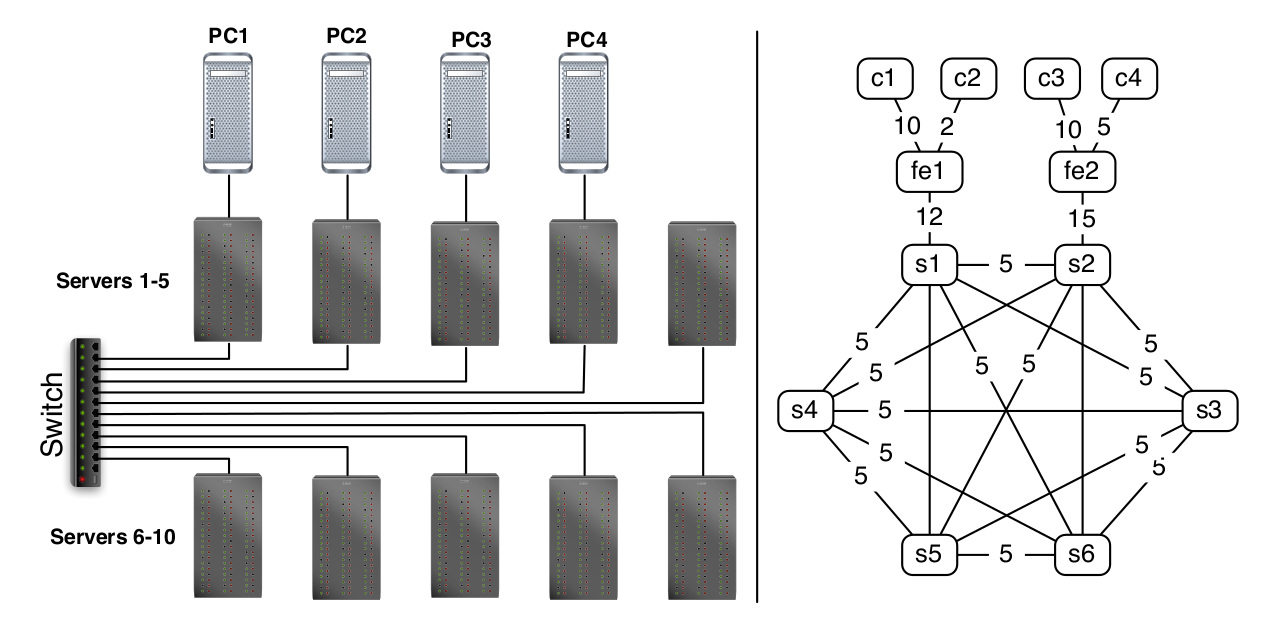
\includegraphics[width=.7\textwidth]{img/esds.png}
\end{center}
\hfill \cite{michel2008optimal}, CPAIOR
\end{frame}

\begin{frame}{Why is it useful to you?}

\alert{As a tool \ldots }

\begin{itemize}
\item If you identify discrete optimization problems in your (self-organizing, autonomic, cloud) application,
you can solve them with reliable tools.
\item Modeling languages provide \emph{easy} access to powerful solvers
\item $\rightarrow$ \emph{independent} of the concrete technology (SAT, CSP, Mathematical Programming)
\end{itemize}

\vspace*{2ex} \pause 
\alert{As a research opportunity \ldots }
\begin{itemize}
\item Studying interactions of complex networks of optimizing agents offers interesting problems (\emph{global systems science})
\item Integration of optimization problems into architectures for decision-making
\item Solving large-scale problems by decomposition through self-organization
\end{itemize}
\end{frame}



\begin{frame}
    \frametitle{Soft Constraint Programming in MiniBrass}
 \alert{Constraint programming} (first half of the tutorial)
    \begin{itemize}
    \item Declarative programming (similar to SQL, Prolog)
    \item Separation of \textbf{model} and \emph{algorithm}
    \item Suitable for combinatorial problems with hard constraints (e.g. physics!)
    \item Modeling language \hFirst{MiniZinc}
    \end{itemize}

    \vspace*{3ex}
    
\alert{Soft constraint programming} (second half of the tutorial)
    \begin{itemize} 
    \item Modeling of \textbf{user preferences}
    \item Find solutions that are \emph{as good as possible} 
    \item What does ``good`` mean?
    \item Modeling language \hFirst{MiniBrass}
     \end{itemize}
\end{frame}

\begin{frame}{Artificial Intelligence: Categories}
\begin{columns}[onlytextwidth,T]
    
    \begin{column}{.5\textwidth}
          
    \hSecond{Data-driven AI}
    \begin{center}
    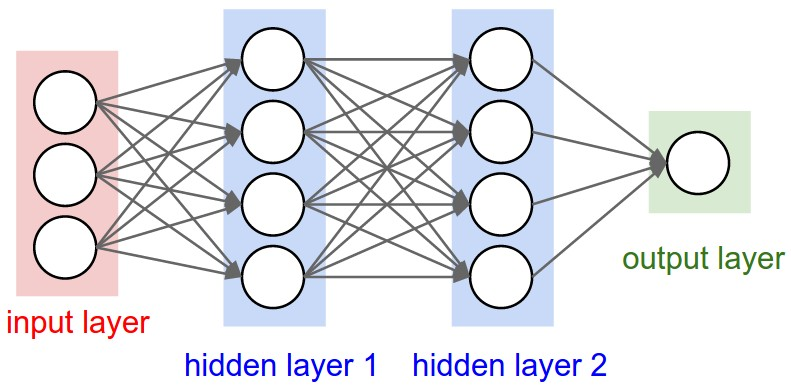
\includegraphics[width=.8\textwidth]{img/neuralnet.jpg}
    \end{center}

    \vspace*{4ex}
    
    \begin{itemize}
    \item Machine Learning
    \item Signal Processing
    \item Computer Vision
    \end{itemize}

    \end{column}
    
    \begin{column}{.5\textwidth}
    \hFirst{Decision-driven AI}
    \begin{center}
    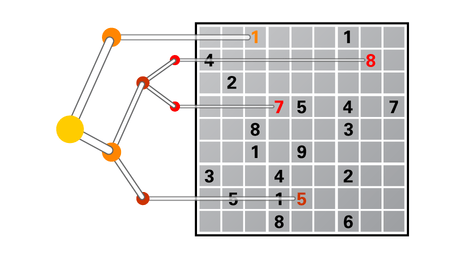
\includegraphics[width=.9\textwidth]{img/discreteopt.png}
    \end{center}
    \begin{itemize}
    \item Constraint Programming
    \item Combinatorial Optimization
    \item Heuristic Optimization
    \item Planning / Scheduling
    \end{itemize}
    
    \end{column}
  \end{columns}
\end{frame}
%


\begin{frame}[fragile]{Our first model}
\begin{lstlisting}
var 0..2: x;
var 0..2: y; 

constraint x < y;

solve maximize x + y;
\end{lstlisting}

\vspace*{2ex}

\url{http://www.minizinc.org}

\vspace*{2ex}

\small
\begin{verbatim}
x = 1;
y = 2;
----------
==========
\end{verbatim}

\end{frame}

\begin{frame}[fragile]{A second example}
\begin{lstlisting}
var 0..2: x; % this notation is shorthand for the set {0,1,2}
var 0..2: y;
var 0..1: z; % {0,1}

% c1
constraint x != y /\ y != z /\ x != z;
% c2
constraint x + 1 = y;

solve satisfy;
\end{lstlisting}
  \vspace*{3ex}
    \alert{Can you give a solution to this problem?} \pause 

\begin{itemize}
\item $\Theta = \{ (x \to 1, y \to 2, z \to \textbf{?}), (x \to 0, y \to 1, z \to \textbf{?}) \}$ satisfy $c_2$; \pause
\item $(x \to 0, y \to 1, z \to ?)$ cannot be extended to a solution since $z$ has to be 0 or 1 $\rightarrow$ has to violate 
$c_1$ \pause
\item Hence, the only solution is $(x \to 1, y \to 2, z \to 0)$
\end{itemize}
\end{frame}

\begin{frame}{Why modeling?}
\begin{enumerate}
\item Once stated (formally) -- solved many times
\begin{itemize}
\item Constraint-Solving
\item SAT -- Boolean Satisfiability
\item MIP -- Mixed Integer Programming
\item Heuristic Optimization -- Genetic etc. 
\end{itemize}
\vspace*{1ex}
\item Efficient and reliable algorithms provided by solvers
\begin{itemize}
\item Same algorithms for a variety of different problems
\item Dedicated algorithms for recurring combinatorial substructures (\texttt{alldifferent})
\end{itemize}
\vspace*{1ex}
\item Prototyping
\begin{itemize}
\item Specification becomes much clearer 
\item Bespoke algorithm for concrete problem can be developed later 
\end{itemize}

\end{enumerate}
\end{frame}

\begin{frame}[fragile]{Modeling in other CS domains}
\begin{lstlisting}[language=sql]
SELECT firstname, lastname
FROM employees 
WHERE age < 30
\end{lstlisting}
\vspace*{1ex}
instead of 
\vspace*{1ex}
\begin{lstlisting}[language=java]
Collection<Person> youngs = new ArrayList<>();
for(Person p : allEmployees) {
  if(p.getAge() < 30)
    youngs.add(p);
}
\end{lstlisting}

\begin{parchment}[Motivation]
\centering 
\alert{Constraint modeling for optimization problems $\approx$ SQL for database access} 
\end{parchment}

\end{frame}

\begin{frame}{NP-Completeness}
\begin{theorem}
The decision problem associated to a constraint satisfaction/optimization problem is NP-complete.
\end{theorem}

\begin{center}
\begin{figure}
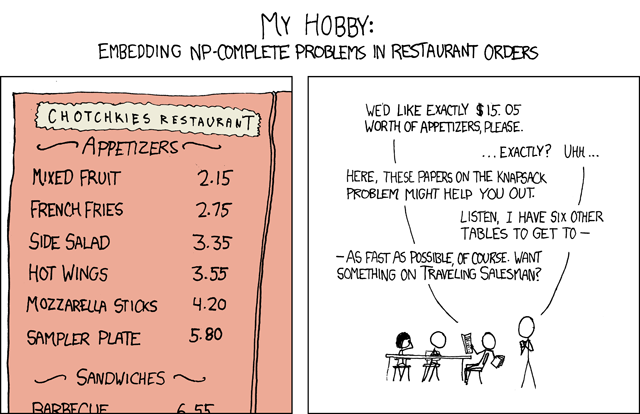
\includegraphics[width=.7\textwidth]{img/np_complete.png}
\caption{\url{https://xkcd.com/287/} }
\end{figure}
\end{center}
\end{frame}

\begin{frame}{Why MiniZinc?}
\begin{parchment}[Rationale]
\centering 
\alert{One modeling language -- many solvers} 
\end{parchment}
\begin{textblock*}{2.cm}[1,1](\textwidth-.5cm,\textheight-1.03cm)


\includegraphics[width=\textwidth]{img/MiniZn_logo.jpg} 

\end{textblock*}
Supported solvers (selection)
\begin{itemize}
\item Gecode (CP)
\item JaCoP (CP)
\item Google Optimization Tools (CP)
\item Choco (CP)
\item G12 (CP/LP/MIP)
\end{itemize}

\end{frame}

\begin{frame}[fragile]{A relevant example \ldots}
\small
\lstinputlisting{models/cakes.mzn}
\end{frame}